\chapter{Preliminaries}
\section{Git}
\textbf{How Conflicts Arise in a GIT-based Branching and Merging Scenario.} Many software projects follow a branching model when using Git, such as the one explained by Giessen [2]. In these models, users create feature branches that provide an environment where new features can be implemented and tested without affecting the end-user version of the software [3]. There are various ways to use branches. A branch can be created for each new feature, in this document called feature-branching. A branch may also be created for each product or variant, in this document called variance-related branching [1]. When a new feature has been implemented in a new branch, the branch needs to be merged into another branch, such as the main branch. Merging is the process of joining two branches together, both in case of two local branches or a local and a remote branch [4]. The local branches are the branches at the client’s copy of the repository, whereas the remote branches are the branches in the remote repository, often on a hosting server such as GitHub. At GitHub, merging is usually done using a pull request. A pull request is made to let the collaborators in the repository know that the commits in a branch are ready to be merged. The collaborators can review the new code and input their feedback until it is finally approved for merging into the end-user branch [5]. When branches are to be merged, conflicts might arise. Conflicts are the problems that prevent git from automatically merging two branches together.

\textbf{Possibilities and limitations of Git.} As git is a fully distributed version control system, one has almost instant access to the complete history of a cloned project. Once a project is cloned, no request limits on project hosting sites are a problem anymore. This makes analyzing a Git-hosted project attractive.

\section{Merging}
\textbf{Code-Clone Management.} Cloning happens during all stages of a software-development process, and it is the responsibility of the developers themselves to make sure that changes between copies of the clones are propagated correctly [1]. Because of this, there are risks that conflicts arise during all stages of the development process.

With the use of a version control system, cloning can be managed in a more smooth way by using branching and merging capabilities [6]. GitHub uses the version control system Git, which maintains a development history for each project. In this history lies the information about when merges have occurred. When cloning features, multiple versions of the same feature exists and their consistency needs to be managed [6].

\textbf{Textual Merging.} The most commonly used merging technique is textual merging [7]. Textual merging is based on the history and on textual differences. It does not make use of any knowledge of the syntax or semantic. One must also distinguish between two-way merging and three-way merging. In two-way merging, only the two conflicting clones are analyzed to resolve the conflict. In three-way merging, also the common ancestor is used, which is more powerful [8].

\textbf{Fast-Forward.} When merging two branches, Git first attempts to perform a so-called fast-forward merge. It is a way of simplifying merges in cases where at least one of the branches points to the common ancestor. Due to that only one version has changed, there can not be any conflicts when merging. In such a case, all that has to be done, is to change both branches to point at the latest commit, see Figure \ref{fig:fastforward}:
\begin{figure}[h]
  \centering
  \begin{subfigure}[b]{0.3\textwidth}
      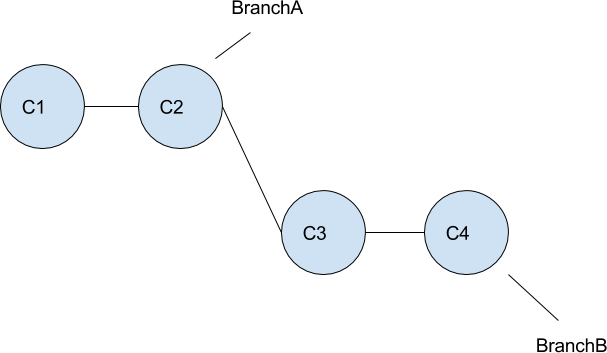
\includegraphics[width=128pt]{figure/ff1.png}
      \caption{Before merge}
      \label{fig:fbranch1}
  \end{subfigure}
  \begin{subfigure}[b]{0.3\textwidth}
      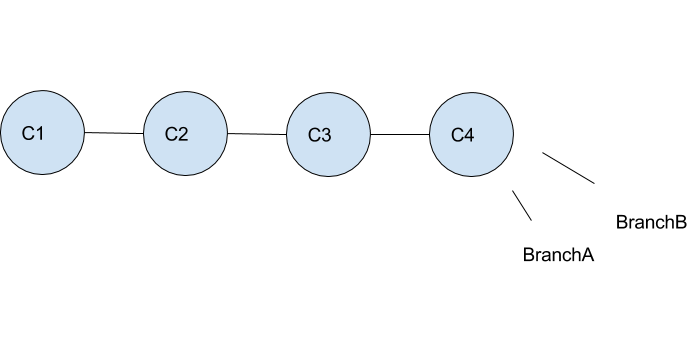
\includegraphics[width=128pt]{figure/ff2.png}
      \caption{After merge}
      \label{fig:fbranch3}
  \end{subfigure}
  \caption{Fast-forward merge}\label{fig:fastforward}
\end{figure}

\textbf{Three-Way Merge.} If fast forward fails, that is, when commits has been made to both branches that are to be merged, Git has to merge all files that the commits contains. This consists of merging the two versions of every file separately, and to be able to know what has changed in the two branches, Git considers both the two versions and their common ancestor. If the files have not been changed at the same places in both branches, Git is able to do this automatically.

\textbf{Parents.} The two commits that are to be merged are called the parents of the merge commit that is created when the merge is made. In this document, the parents will often be referred to as the left- and the right version. The left version is the commit that was checked out at the time of the merge, and the right version is the commit that is being merged into the currently checked out branch. For instance, when pulling the remote branch to merge with the local branch, the left version will be the local version and the right version will be the remote version that is being pulled.

\textbf{Git Conflicts.} If the two commits, that are to be merged, have made changes to the same place in a file, Git will not be able to merge the two versions automatically. This is called a Git conflict. When a Git conflict occurs, Git will output the conflicting file paths in the commit message, which the tool parses. When resolving conflicts, it is usually done by manually merging the conflicting lines of the local file (the file in the current checked out branch) with the file of the remote file (the file of the branch which is being merged into the current checked out branch) and the common ancestor file (the original file before it was changed in the local- and remote branches).

\textbf{Semistructured Merging.} Furthermore, there exist merge tools that use approaches other than textual merging, such as syntactic- and semantic merging, which have language specific knowledge [9] and do not only compare lines of text. A combination of both textual merging, syntactic and semantic merging is called semi-structured merging [7]. Other studies have proved that the use of semistructured merge decreases the number of conflicts significantly. Cavalcanti et al. proves that semistructured merge can reduce the number of conflicts by 55\% [10]. Our work is different in that we instead of proposing a new conflict resolution technique, we are interested in how developers resolve conflicts arising from different variants of features or projects.

\section{Conflict Patterns}
During merging, several types of conflict patterns might occur. In her study, Accioly [11] identifies numerous conflict patterns, using her developed tool Conflicts Analyzer.

In her study, Accioly lists conflict patterns that describe types of conflicts that might arise during a merge. The study uses a semi-structured merge tool, called SSMerge, which performs merges by first constructing Feature-Structured Trees, a.k.a FST, for the two versions of the file that is to be merged. The two trees are then merged using superimposition. This is possible due to that the order of methods and class variables inside a class does not matter. Code segments where the ordering matters in Java, ie. method- and constructor bodies, cannot be merged this way and are therefore placed in the leaves of the tree [7]. It is conflicts that concern these leaves that are of interest to this study.

The conflict patterns are derived from the conflicts that SSMerge can detect [11]. Table \ref{table:conflictpatterns} lists the patterns from Accioly’s study that is listed in the online appendix:\\% HELLO FERRET, INSERT FOOT NOTE FROM THESIS REKÅT
\begin{table}
\caption{Conflict patterns}\label{table:conflictpatterns}
\begin{tabular}{| l | p{10cm} |}
\hline
\multicolumn{1}{c}{\textbf{Pattern}} & \multicolumn{1}{c}{\textbf{Description}}\\
EditSameMC & Different edits to the same area of the same method or constructor\\
SameSignatureCM & Methods or constructors added with the same signature and different bodies\\
EditSameFd & Different edits to the same field declaration\\
AddSameFd & Field declarations added with the same identifiers and different types of modifiers\\
ModifierList & Different edits to the modifier list of the same type declaration (class, interface, annotation or enum types)\\
ImplementsList & Different edits to the same implements declaration\\
ExtendsList & Different edits to the same extends declaration\\
DefaultValueA & Different edits to the same annotation method default value
\end{tabular}
\end{table}
From Table \ref{table:conflictpatterns}, it is the EditSameMC- and SameSignatureCM patterns that concern the leaves of the tree.


